Another way to detect the formation of shocks computationally is by
measuring entropy.  An entropy function for \eqref{nel_pde} is the total energy:
\begin{align}
  \eta(u,\epsilon,x) = \frac{1}{2}\rho(x)u^2 + \int_0^\epsilon \sigma(s,x)ds.
\end{align}
It is straightforward to see that $\eta$ is conserved for smooth solutions:
\begin{align*}
  \frac{d}{dt} \int_{-\infty}^\infty \eta dx & = \int_{-\infty}^\infty \eta_t dx \\
    & = \int_{-\infty}^\infty \left(\rho(x) u u_t + \frac{d}{dt}\int_0^{\epsilon(x,t)} \sigma(s,x) ds \right) dx \\
    & = \int_{-\infty}^\infty \left(\rho u u_t + \sigma(\epsilon,x)\epsilon_t\right) dx \\
    & = \int_{-\infty}^\infty \left(u\sigma_x + \sigma u_x\right) dx = \int_{-\infty}^\infty (\sigma u)_x dx = 0.
\end{align*}
However, when shocks form the entropy of the physically correct
vanishing-viscosity solution will decrease.  Since our numerical
methods are designed to compute the vanishing-viscosity solution,
the numerical entropy will also tend to decrease when shocks form.
In this section we study the evolution of entropy in computational solutions.

In \Fig{entropy_1}, we show the evolution of entropy over time for 
an initial gaussian stress perturbation
in a medium with $\rho_A=K_A=1$ and $\rho_B=K_B=Z_B$, for
varying values of $Z_B$.  In each case, the entropy is normalized to be
unity at time zero.  The case $Z_B=1$ corresponds to a homogeneous
medium, and the entropy decays rapidly once a shock forms.  
For $Z_B=2$, the entropy evolution indicates that shock formation is
delayed and the resulting shocks are weaker.
For $Z_B=4$, the entropy is nearly constant over the duration
of the simulation.

\begin{figure}
\centerline{
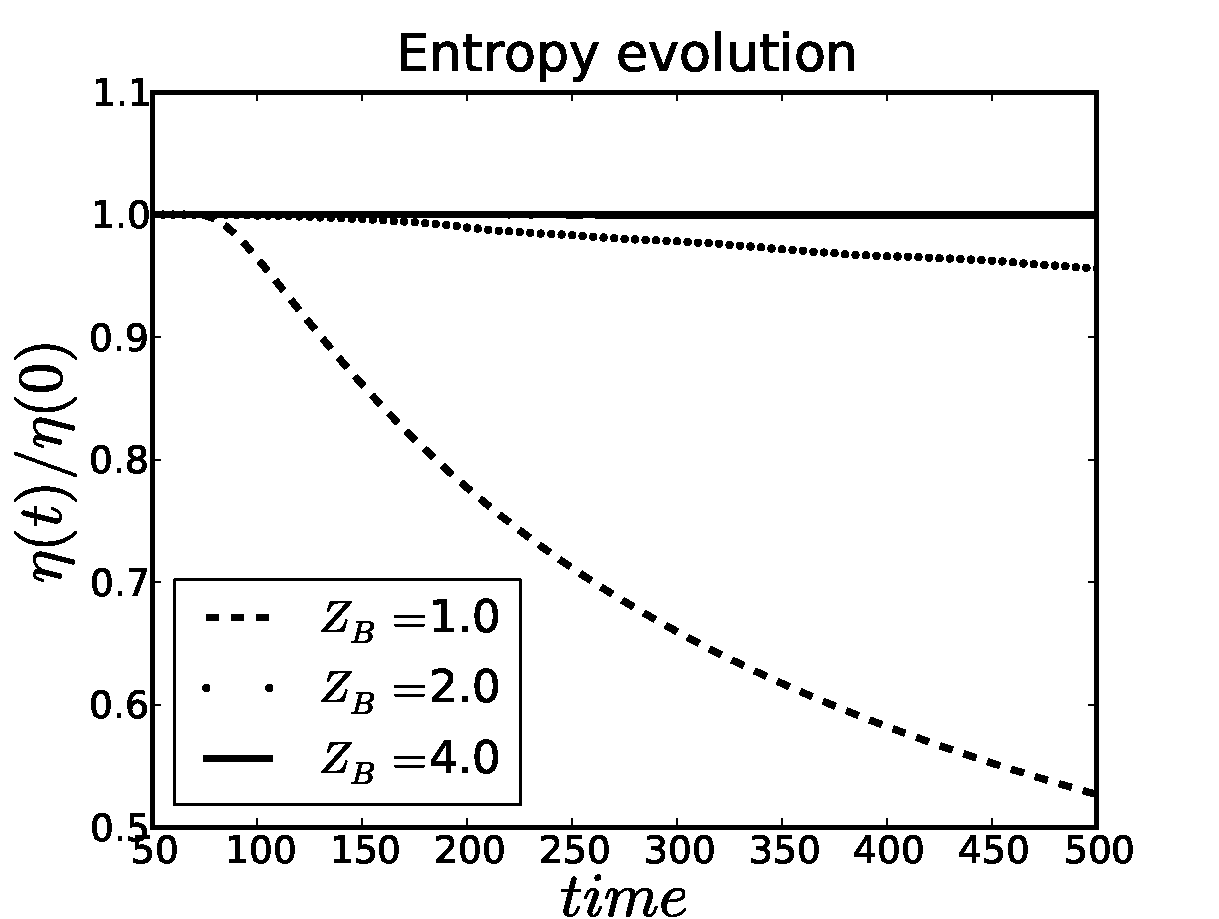
\includegraphics[width=4in]{figures/entropy.pdf}}
\caption{Entropy evolution in time for media with various impedance
ratios.  In this test, the density and bulk modulus of layer B were 
varied simultaneously and are equal to $Z_B$ in each case.\label{fig:entropy_1}}
\end{figure}

Numerical dissipation can also lead to a loss of entropy in the 
computational solution.  Using a first-order method, the entropy evolution
is entirely dominated by this effect.  For the higher order numerical
methods employed in this paper, we have found that entropy may 
numerically increase or decrease
depending on how agressive the limiter is.  Overcompressive numerical 
limiters can lead to (unphysical) entropy production.  However, all
numerical effects on entropy evolution appear to decrease rapidly
with grid resolution, as shown in \Fig{entropy_lims}, which indicates
the relative entropy loss versus grid resolution at $T=500$ for $Z_B=4$.
Among the limiters implemented in Clawpack, the smallest change 
in entropy is generally produced by the van Leer limiter (for sufficiently
fine grids).
The van Leer limiter is used in all subsequent Clawpack simulations 
in this paper.  Using SharpClaw with fifth-order WENO reconstruction, 
we find that the entropy errors are much smaller than for any of the 
Clawpack limiters, especially on the finer grids.

We remark that this test might be taken as a measure of the 
 dissipativity of a given limiter.  For instance, note that
the results in \Fig{entropy_lims} for Minmod and Superbee suggest that
they are dissipative and over-compressive, respectively.
It is interesting to note that, by this measure, the MC limiter
is somewhat over-compressive, while the van Leer limiter is somewhat
dissipative. Fifth-order WENO is neutrally-compressive.  That is, the
entropy fluctuates slightly around the initial value, but is roughly constant
in time if averaged over short intervals.

\begin{figure}
\centerline{
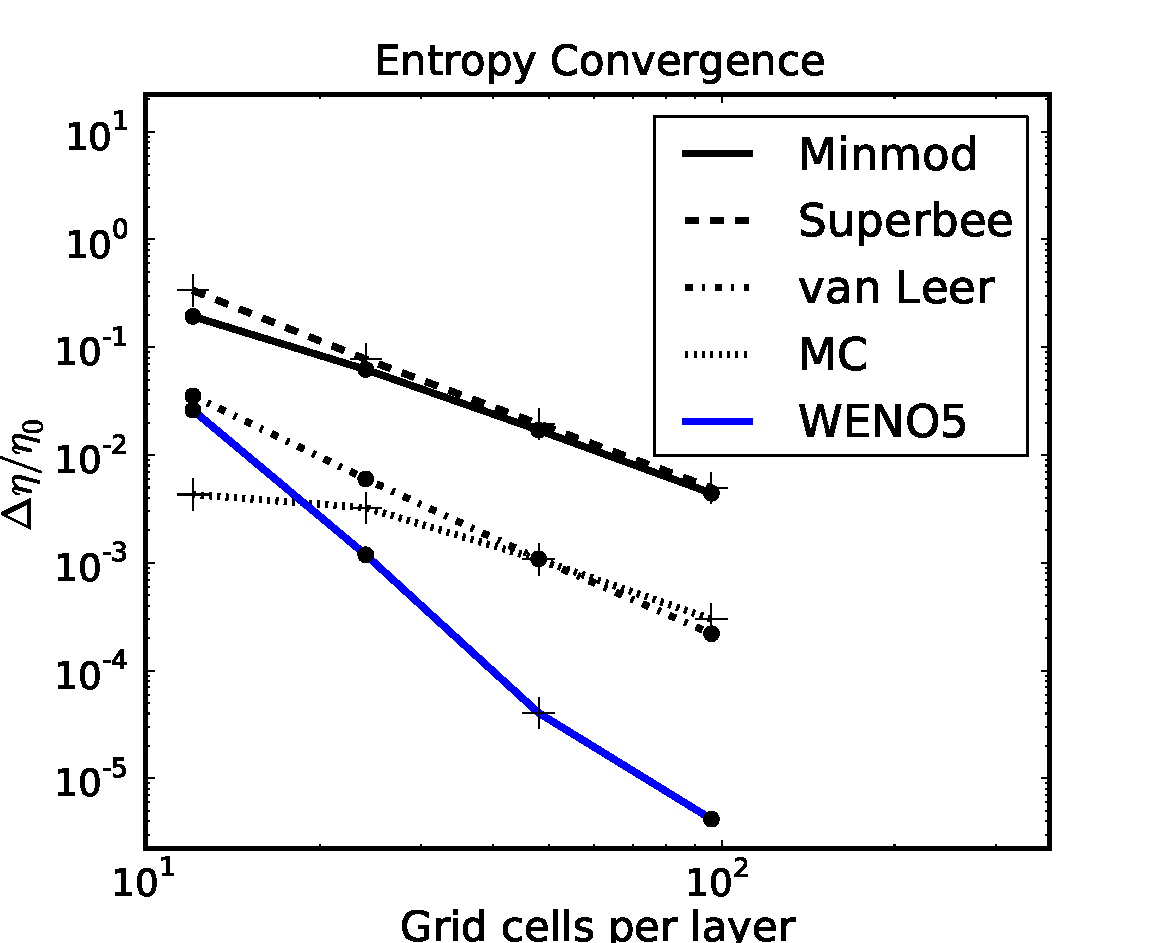
\includegraphics[width=4in]{figures/limiter_entropy_convergence.pdf}}
\caption{Entropy change up to $T=500$ versus number of grid cells per
medium layer for the four limiters implemented in Clawpack.  Here $Z_B=4$.
Plus signs ('+') indicate cases for which the entropy has increased, while
filled circles
indicate cases for which the entropy has decreased.\label{fig:entropy_lims}}
\end{figure}

Due to numerical dissipation (or compression), it is impossible 
to completely rule out physical loss of entropy.  Instead, we can bound the 
possible loss of entropy through use of very fine spatial resolution.
For sufficiently fine grids, we have noticed that the small
numerical entropy fluctuations are nearly time-reversible.  That is,
if we run the time-reversibility experiment of the last section and
consider the entropy at corresponding early and late times, the 
difference is much smaller than the (already small) difference between
the entropy at either time and the initial entropy.  This allows us
to probe the degree to which entropy is
conserved for different impedance contrasts.  

In Figure \ref{fig:trent}, we plot the difference in entropy 
values at times $t=50$ and $t=450$ (using a final time of $T=500$), for 
SharpClaw solutions on fine grids.
We observe that the change in entropy generally 
gets smaller as the impedance contrast increases and as the resolution
of the simulation increases.  For a given grid, 
the entropy change apparently diminishes until it reaches the level of numerical
errors.  For impedance contrast greater than
2.5, the entropy change on the finest grid is less than $10^{-7}$.
Similar results are obtained with Clawpack, although much finer
resolution is required to resolve the small losses of entropy \cite{alghamdipetclaw}.

\begin{figure}
\centerline{
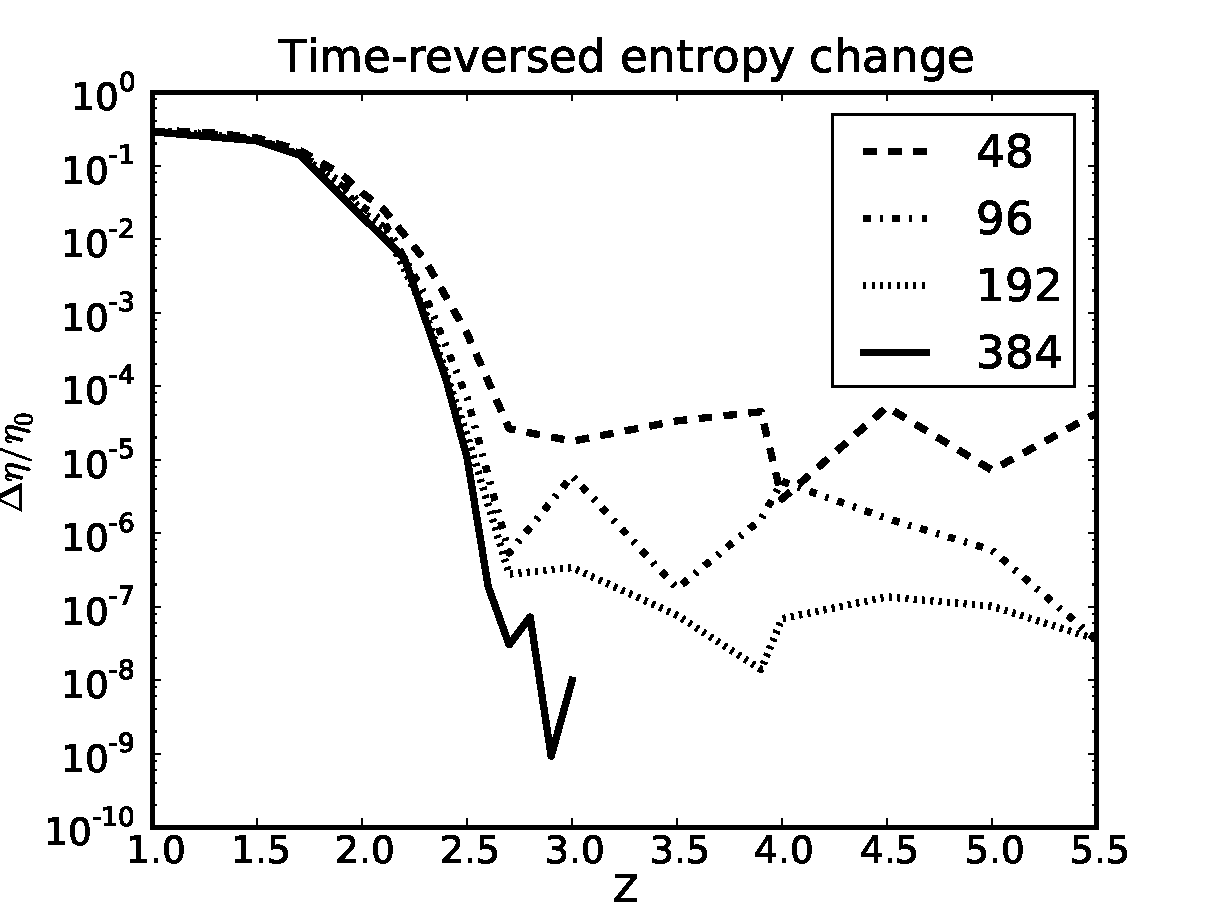
\includegraphics[width=4in]{figures/trent_all.pdf}}
\caption{Change in entropy for LY media with increasing impedance contrast.
The different plots correspond to differing spatial resolutions; the
number of cells per material layer is indicated in the legend.\label{fig:trent}}
\end{figure}


%One possibility for future work is the development of exactly 
%entropy-conserving schemes for this variable-coefficient system.
%This may allow one to rule out the formation of shocks down to
%the level of roundoff errors.

%In all of the test cases so far, $\rho_B$ and $K_B$ have been
%varied simultaneously.  We now consider a wider test by varying
%each separately.  In order to generate a 'fair' comparison, we
%fix (approximately) the entropy of the initial condition.  Also,
%we employ an initial condition designed to generate a right-moving
%train of solitary waves.  Specifically, our initial condition is
%\begin{align*}
%u_0(x) & = -0.2 \exp\left(-\frac{(x-75)^2}{100}\right) \\
%\sigma_0(x) & = \left(1-\frac{\Zmean}{2}u_0(x)\right)^2 - 1.
%\end{align*}
%We also scale the simulation final time inversely with
%the homogenized linear sound speed, solving up to $T=625/\cmean$.
%The purpose of this is to compare solutions after the waves
%have passed through a similar number of layers of the medium.
%Results are shown in \Fig{entropy_2} and \Fig{entropy_3}.
%
%\begin{figure}
%\centerline{
%\includegraphics[width=4in]{figures/entropy_tests_57600.pdf}}
%\caption{Change in entropy for media with various values
%of $\rho_B,K_B$.  \label{fig:entropy_2}}
%\end{figure}
%
%\begin{figure}
%\centerline{
%\includegraphics[width=4in]{figures/entropy_tests_vsZ_57600.pdf}}
%\caption{Change in entropy versus impedance mismatch.\label{fig:entropy_3}}
%\end{figure}


